\documentclass[uplatex,dvipdfmx,a4paper,twocolumn,base=11pt,jbase=11pt,ja=standard]{bxjsarticle}  % 環境に合わせて変更してください

\usepackage{ipsj}
\usepackage{color}

%追加パッケージ
\usepackage{enumerate}
\usepackage{url}
\usepackage{graphics}
\usepackage{caption}
%\usepackage[dviout]{graphicx}
%\usepackage[dvipdfmx]{graphicx}
\usepackage{graphicx}

\newcommand{\todo}[1]{\colorbox{yellow}{{\bf TODO}:}{\color{red} {\textbf{[#1]}}}}

\title{README修正内容に関連する\\ソースコード変更コミット追跡への試み}{Toward tracking source code change commits related to README revision}
\author{和歌山大学}{白﨑 優奈}{Shirasaki Yuna, Wakayama University}
\author{和歌山大学}{伊原 彰紀}{Akinori Ihara, Wakayama University}
\author{和歌山大学}{石岡 直樹}{Naoki Ishioka, Wakayama University}

\begin{document}
\maketitle


%================
%1
\section{はじめに}
%================

%hogehoge(背景,動機とか)

多くのソフトウェア開発プロジェクトでは,ソフトウェアの機能,使用方法などを開発者や利用者に発信するため,ソフトウェアドキュメントとしてREADMEを公開している.ソフトウェア開発の中でもGitHubを利用するオープンソースソフトウェア (OSS) 開発では,開発への参加方法,各機能の概要などもREADMEに記述しており,READMEはリポジトリのトップページに提示される重要なドキュメントとなっている.

% (プロプライエタリソフトウェアでは,定期的なリリースの際にソフトウェアとドキュメントを同時に公開する.一方で)
OSSプロジェクトは,実装中のソースコードを逐一公開しているため,ソースコードの更新に伴ってREADMEの更新が期待される.しかし従来研究ではソースコードとREADMEが紐付けられていないため,ソースコードとREADMEがどのように共進化しているか明らかでない.また,開発者はソースコードとREADMEを同一コミットで更新していないこともあり,READMEの更新が必要となったソースコードの変更コミットを紐付けることは容易でない.

本研究は,README更新の追従性を確認するため,ソースコードとREADMEの変更内容に共通して含まれる文字列に基づいて関連付ける方法を提案する.特にREADMEの変更と,関連づけられたソースコードのコミットとの時間差を分析することで,プロジェクトにおけるREADMEの記述方針を明らかにする.\todo{今後は,記述方針がソフトウェア品質や効率にどう影響するか明らかにしたいなぁ..ここまではこの論文で書けないけど.}

%================
%2
\section{分析}
%================

%================
%2.1
\subsection{分析手法}
%================
%hogehoge(分析を行うためにどんな準備をしたか(スニペット削除とか))

%fugofugo(なぜその準備をしたのか(コードがあったらよろしくないとか))





の両方に同じ文字列
READMEの変更に関連することが示唆されるソースコードの変更コミットを特定する.具体的には,READMEの更新\todo{更新には追加,変更,削除を含むよね?}された文字列と,各コミットにおいて変更されたソースコード中の文字列をそれぞれ抽出し,同じ文字列を含むREADMEとソースコードを関連づける.ソースコードファイル中から記号削除,NLTKを用いて形態素解析により名詞のみを抽出する.同様の手法で,README変更コミットで追加されたREADMEから名詞のみを抽出する.\todo{READMEは変更内容のみではないの?README全体?}

% READMEの変更を誘発するソースコードの変更コミットを確認するために,READMEと,各コミットで追加された文章をデータ整形する.\todo{各コミットで変更されたソースコードに含まれる文字列を抽出する}.本研究では,READMEが変更されたコミット,および前後のコミットにおいて変更されたソースコードを対象とし,ソースコードファイル中から記号削除,NLTKを用いて形態素解析により名詞のみを抽出する.

%具体的には,ソースコードファイル中の
%
%\vspace{-2mm}
%\begin{enumerate}
%    \item READMEが変更されたコミットについて,各コミットで追加された文章を抽出
%    \item 正規表現を用いて,記号の削除
%    \item NLTKを用いて,説明文の分かち書き
%    \item NLTKを用いて,名詞を抽出
%    \item 全コミットを対象に,追加されたソースコードに同様の処理
%\end{enumerate}
%
%以上の方法で,READMEの変更コミットで追加された文章に含まれる名詞,全コミットで追加されたソースコードに含まれる名詞が得られる.

%抽出した単語に一致単語があるかを比較分析する.比較ペアは,README変更コミットで追加された単語と,その前後Nコミットのコード変更で追加された単語である.一定数以上の単語の一致があれば,そのコード変更はREADMEの変更を誘発したとする.

% 抽出した単語に一致単語があるかを比較分析する.\todo{上記では,READMEからの収集方法について書いていないように思いますが....}比較ペアは,README変更コミットで追加された単語と,その前後Nコミットのコード変更で追加された単語である.一定数以上の単語の一致があれば,そのコード変更はREADMEの変更を誘発したとする.


%================
%2.3
\subsection{ケーススタディ}
%================
%hogehoge(どんなデータセット使ったか)

%fugofugo(そこからどんなデータをどうやって集めたか)

本論文では,READMEが英語で記述され,他のリポジトリに比べて頻繁に保守している2つのプロジェクト (aliyun-openapi-nodejs-sdk, js-multiaddr) を対象とする.

%hogehoge(どんな結果が得られたか,図とかを一緒に載せる)

図\ref{fig:aliyun}と図\ref{fig:multiaddr}は,それぞれのプロジェクトを対象に,READMEの変更コミットの前後10コミットそれぞれにおいて,READMEにおいて変更された文字列を含む頻度を計測した結果である.横軸はREADMEを変更したコミットを0とする前後のコミット位置を示し,縦軸はソースコード中に含むREADMEにおいて変更された文字列の数を示す.紙面の都合上,XXを変更したREADMEの変更箇所をケーススタディとして示す.\todo{READMEが変更されたコミットは他にもあったと思うけど,なぜこのコミットを選んだ?}

%で追加された単語とその前後10コミットで追加された単語を比較し,一致単語があるならば一致数を加算し,README変更コミットやその前後コミットにおいて,関連単語がいくつあるのかを示している.縦軸は一致単語数,横軸はREADME変更コミットを0とした前後のコミットを示す.

%fugofugo(結果からの考察)
%分析を行った結果次のような結果が得られた.

%図1はaliyun-openapi-nodejs-sdkを,図2はjs-multiaddrを対象に分析した結果である.
% \documentclass{jsarticle}
% \usepackage{bardiag}
% \begin{document}
% \renewcommand{\betweenticks}{50}
% \bardiagrambegin{9.5}{350}{1}{2}{1cm}{0.02cm}
%     % \drawlevellines
%     % \baritem{-20}{23}{blue}
%     % \baritem{-19}{5}{blue}
%     % \baritem{-18}{2}{blue}
%     % \baritem{-17}{24}{blue}
%     % \baritem{-16}{24}{blue}
%     % \baritem{-15}{27}{blue}
%     % \baritem{-14}{21}{blue}
%     % \baritem{-13}{20}{blue}
%     % \baritem{-12}{7}{blue}
%     % \baritem{-11}{2}{blue}

%     \baritem{0}{23}{blue}
%     \baritem{1}{5}{blue}
%     \baritem{2}{2}{blue}
%     \baritem{3}{24}{blue}
%     \baritem{4}{24}{blue}
%     \baritem{5}{27}{blue}
%     \baritem{6}{21}{blue}
%     \baritem{7}{20}{blue}
%     \baritem{8}{7}{blue}
%     \baritem{9}{2}{blue}
% \bardiagramend{\large README変更コミットの前後のコミット}{\large 一致単語数}
% \end{document}

%-----------------------
\begin{figure}[t]
\begin{center}
%\includegraphics[width=6cm]{IPSJ202303_Shirasaki/draft/use_aliyun.pdf}
\includegraphics[width=0.7\linewidth]{use_aliyun.pdf}
\vspace{-5mm}
\caption{aliyun-openapi-nodejs-sdkにおける各コミット中のREADMEの変更単語数}
\label{fig:aliyun}
\end{center}

\vspace{-8mm}

\begin{center}
%\includegraphics[width=6cm]{IPSJ202303_Shirasaki/draft/use_js.pdf}
\includegraphics[width=0.7\linewidth]{use_js.pdf}
\vspace{-5mm}
%\caption{js-multiaddrを対象とした,各コミットごとのREADMEとコードに含まれる一致単語数}
\caption{js-multiaddrにおける各コミット中のREADMEの変更単語数}
\label{fig:multiaddr}
\end{center}
\vspace{-12mm}
\end{figure}
%-----------------------

\noindent\texttt{aliyun-openapi-nodejs-sdk: }図\ref{fig:aliyun}のA(0)においてREADMEが更新され,1コミット前のA(-1)とA(0)のソースコード変更がREADMEの更新に関連していることが示唆される.A(-1)とA(0)のソースコードでは\todo{Xの変更}が行われ,READMEには\todo{XXの内容が追記?削除?変更?}されている.このコミットでは,実装後にREADMEが更新されたことが示唆される.

%たコミットで,更新されたREADMEと変更されたソースコードにおいて一致した単語の数を表している.
%A(-1)はREADME更新の2つ前のコミットで,A(0)で更新されたREADMEと,このコミットで変更されたソースコードにおいて一致した単語の数を表している.
%
%A(0)の一致単語には\todo{書きます}が見られ,実際にREADMEに反映された単語が多く含まれていた.
%A(-1)でも実際にREADMEに反映された単語が多く含まれていた.ここから,このリポジトリでは,READMEを連続して更新していることがわかった.また,A(-1)を含むREADME更新以前のコミットに一致単語が多いことから,ソースコードをまとめて変更してからその変更をREADMEに反映させて開発していると考えられる.


% 図1より,README変更コミットとその前のコミットで,一致単語が多くみられた.ここから,README変更に関連のあるソースコードは,READMEとほぼ同時に変更される分量が多いことがわかった.

\noindent\texttt{js-multiaddr: }図\ref{fig:multiaddr}のB(0)においてREADMEが更新され,2コミット後のB(2)とB(0)のソースコード変更がREADMEの更新に関連していることが示唆される.A(2)とA(0)のソースコードでは\todo{Xの変更}が行われ,READMEには\todo{XXの内容が追記?削除?変更?}されている.このコミットでは,実装前にREADMEが更新されたことが示唆される.



%図\ref{fig:multiaddr}のB(0)はREADMEが更新されたコミット,B(2)はREADME更新の2つ後のコミットで,READMEとソースコードにおいて一致した単語の数を表している.
%
%B(0)の一致単語にはmultiaddrなどの変数名\todo{もうちょっと書きます}が見られ,実際にREADMEに反映された単語が含まれていた.
%B(2)でも実際にREADMEに反映された単語が多く含まれており,目視での確認を通して,このリポジトリではREADMEを1コミットおきに更新する傾向があることがわかった.また,B(2)を含むREADME更新以後のコミットに一致単語が多いことから,READMEを更新した後に,何度かにわけてソースコードを変更していると考えられる.
%
%以上から,ソースコードの変更を反映させるREADMEの更新はコード変更の前にも後にもおこなわれており,コード変更と同時に行われることが多いとわかった.
%
%\todo{2つのグラフの閾値をA:5,B:10にして結果とすることを検討中.README前,README後の傾向がより顕著になるため.文章を検討中のため未記述}
% \todo{2つの結果からわかることの記述}


% 以下使わない
% また図2は,README変更コミットで追加された単語とその前後20コミットで追加された単語を比較し,10以上の一致単語があるならば一致する(1),一致単語が10未満なら一致しない(0)として,各コミットの一致の有無を示したグラフである.
% 図2より,README変更前の方が,README変更後よりも密にソースコードの変更がみられる.ここから,ソースコードを変更してから,まとめてREADMEが変更されることが多いことがわかった.


%--------------------------------グラフ

%--------------------------------

%================
%3
\section{おわりに}
%================

%hogehoge(今回の研究のまとめとか)

%fugofugo(今回研究から得られたことを踏まえて今後どう発展させていくか)

%42(どんな研究をしていくつもりなのか的な)
%今回の研究のから hogehoge-fugofugoである.

本論文では,READMEがソースコードの変更を追従しているかを確認するため,各ファイルの単語を比較した.
% 分析の結果,README更新の前からREADMEが更新されるまでの間に,READMEに関連のあるソースコードが多く変更されていることがわかった.
分析の結果,READMEの更新は,ソースコード変更の前と後のいずれの時期でも変更されることがあり,READMEの内容に応じて追従するタイミングが異なると考える.
今後は,READMEとソースコード変更内容によるREADMEの追従性違いを明らかにし,READMEの追従性によるソフトウェア品質への影響を示す.また,READMEの自動更新タイミングについても検討する.



%================
\section*{謝辞}
%================


%================
% \section*{参考文献}
%================
%[1]Shohei IKEDA, Akinori IHARA, Raula Gaikovina KULA, and Kenichi MATSUMOTO : An Empirical Study ofREADMEcontents for JavaScript Packages : IEICE TRANS. INF. and SYST., VOL.E102–D, NO.2 FEBRUARY 2019

%[2]JINHAN KIM, SANGHOON LEE, and SEUNG-WON HWANG, SUNGHUN KIM : Enriching Documents with Examples: A Corpus Mining Approach : ACM Trans. Inf. Syst. 31, 1, Article 1 (January 2013)

%[3]Noela Jemutai Kipyegen and William P. K. Korir : Importance of Software Documentation : IJCSI International Journal of Computer Science Issues, Vol. 10, Issue 5, No 1, September 2013 
\todo{メモ:少し削る,グラフ軸名記入}

%================

\bibliographystyle{ipsjunsrt}
\bibliography{bibfile}

\end{document}
